\section{Experiments}
\label{sec:experiments}
We use Fetch push, reach and pick and place
tasks~\citep{plappert201802multigoalrl} in our experiments:
%
\begin{description}
  \item[Fetch-Reach] The tip of a robotic arm reaching a desired location.
  \item[Fetch-Push] A robotic arm pushing a block to a desired location.
  \item[Fetch-Slide] A robotic arm sliding a puck to a desired location.
\end{description}%
% 

%
\begin{figure}%
  \def\frac{0.24}
  \rotatebox{90}{\hspace{2em}\color{blue}{\tiny Fetch Reach}}%
  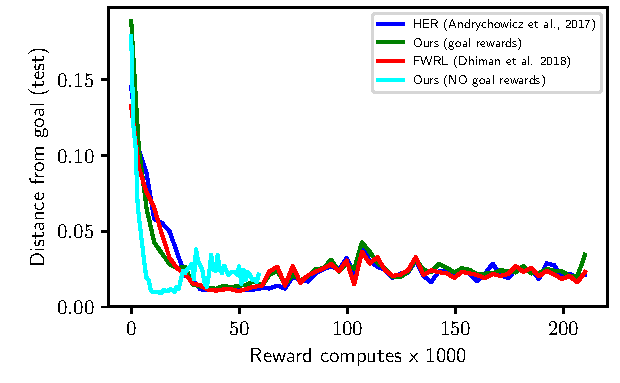
\includegraphics[width=\frac\columnwidth]{media/res/6efc1de-path_reward_low_thresh_chosen-FetchReachPR-v1-dqst/reward_computes-test/ag_g_dist.pdf}%
  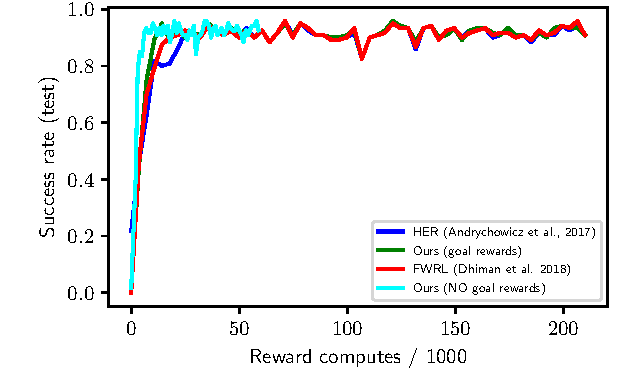
\includegraphics[width=\frac\columnwidth]{media/res/6efc1de-path_reward_low_thresh_chosen-FetchReachPR-v1-dqst/reward_computes-test/success_rate.pdf}%
  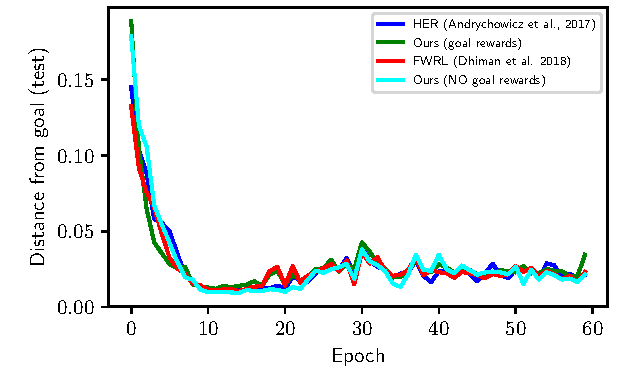
\includegraphics[width=\frac\columnwidth]{media/res/6efc1de-path_reward_low_thresh_chosen-FetchReachPR-v1-dqst/epoch-test/ag_g_dist.pdf}%
  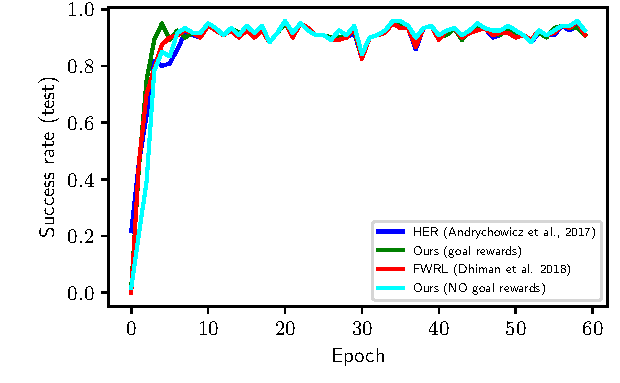
\includegraphics[width=\frac\columnwidth]{media/res/6efc1de-path_reward_low_thresh_chosen-FetchReachPR-v1-dqst/epoch-test/success_rate.pdf}\\
  \rotatebox{90}{\hspace{2em}\color{blue}{\tiny Fetch Push}}%
  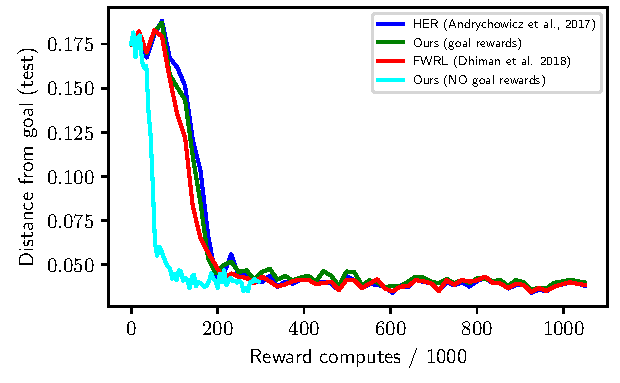
\includegraphics[width=\frac\columnwidth]{media/res/6efc1de-path_reward_low_thresh_chosen-FetchPushPR-v1-dqst/reward_computes-test/ag_g_dist.pdf}%
  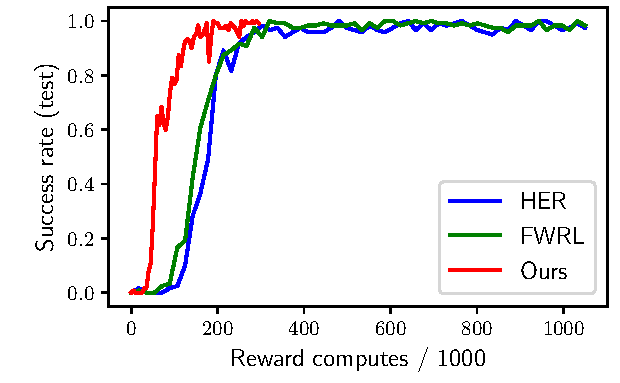
\includegraphics[width=\frac\columnwidth]{media/res/6efc1de-path_reward_low_thresh_chosen-FetchPushPR-v1-dqst/reward_computes-test/success_rate.pdf}%
  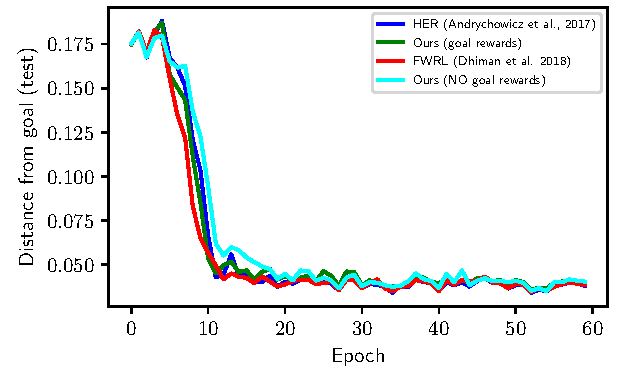
\includegraphics[width=\frac\columnwidth]{media/res/6efc1de-path_reward_low_thresh_chosen-FetchPushPR-v1-dqst/epoch-test/ag_g_dist.pdf}%
  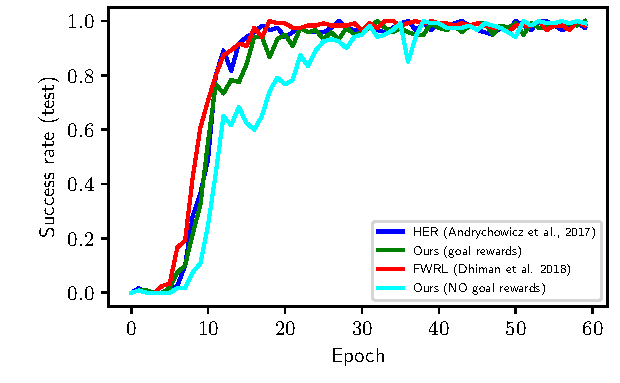
\includegraphics[width=\frac\columnwidth]{media/res/6efc1de-path_reward_low_thresh_chosen-FetchPushPR-v1-dqst/epoch-test/success_rate.pdf}\\
  \rotatebox{90}{\hspace{2em}\color{blue}{\tiny Fetch Slide}}%
  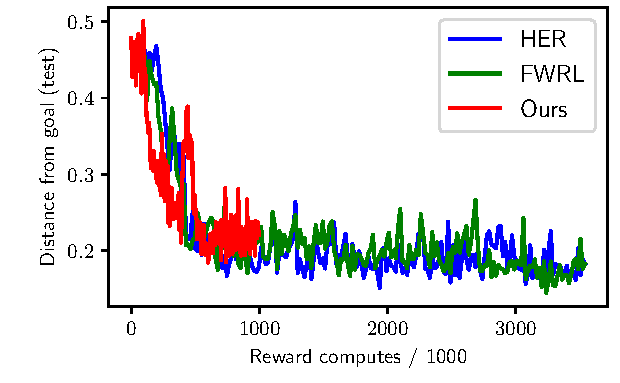
\includegraphics[width=\frac\columnwidth]{media/res/6efc1de-path_reward_low_thresh_chosen-FetchSlidePR-v1-dqst/reward_computes-test/ag_g_dist.pdf}%
  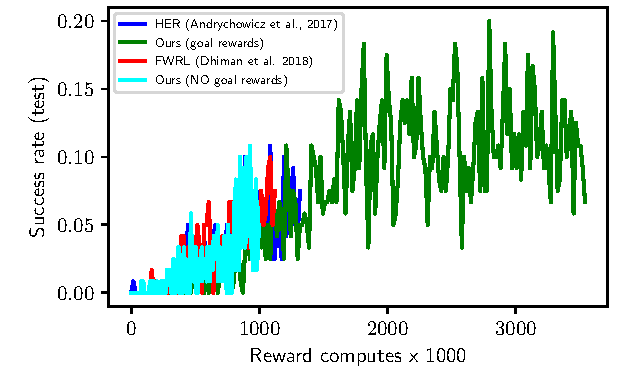
\includegraphics[width=\frac\columnwidth]{media/res/6efc1de-path_reward_low_thresh_chosen-FetchSlidePR-v1-dqst/reward_computes-test/success_rate.pdf}%
  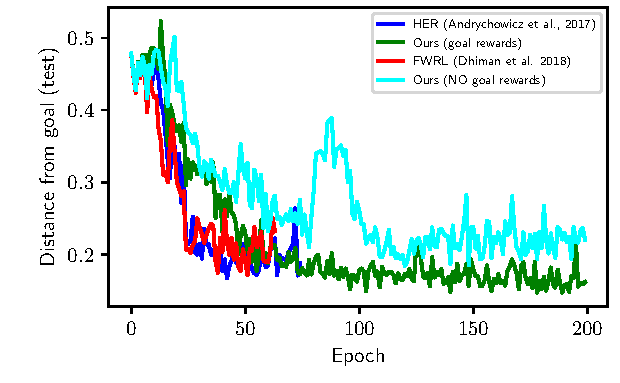
\includegraphics[width=\frac\columnwidth]{media/res/6efc1de-path_reward_low_thresh_chosen-FetchSlidePR-v1-dqst/epoch-test/ag_g_dist.pdf}%
  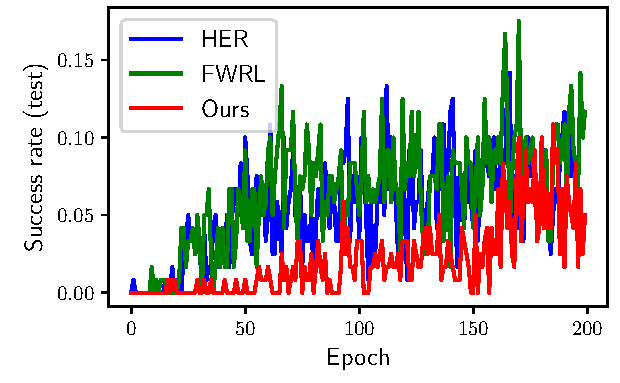
\includegraphics[width=\frac\columnwidth]{media/res/6efc1de-path_reward_low_thresh_chosen-FetchSlidePR-v1-dqst/epoch-test/success_rate.pdf}\\
  \rotatebox{90}{{\tiny \hspace{1em} \color{blue}{Fetch Pick And Place}}}%
  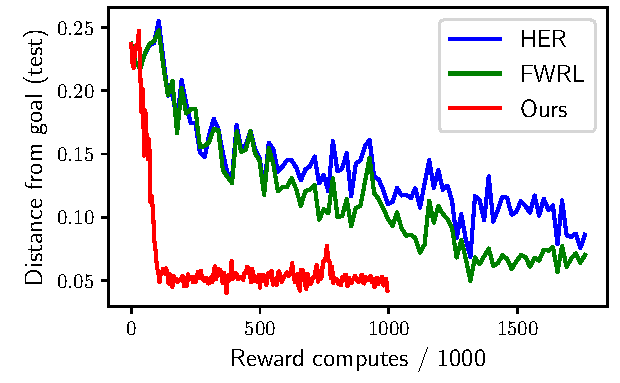
\includegraphics[width=\frac\columnwidth]{media/res/6efc1de-path_reward_low_thresh_chosen-FetchPickAndPlacePR-v1-dqst/reward_computes-test/ag_g_dist.pdf}%
  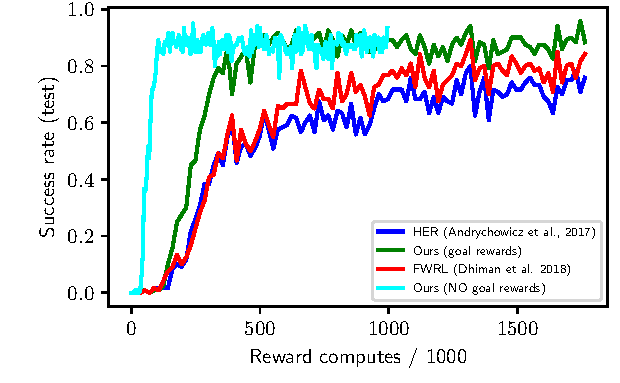
\includegraphics[width=\frac\columnwidth]{media/res/6efc1de-path_reward_low_thresh_chosen-FetchPickAndPlacePR-v1-dqst/reward_computes-test/success_rate.pdf}%
  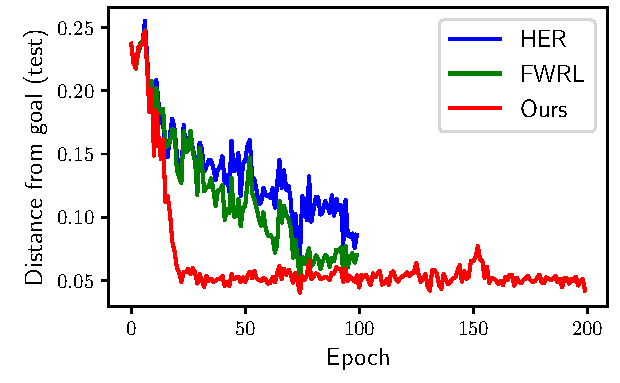
\includegraphics[width=\frac\columnwidth]{media/res/6efc1de-path_reward_low_thresh_chosen-FetchPickAndPlacePR-v1-dqst/epoch-test/ag_g_dist.pdf}%
  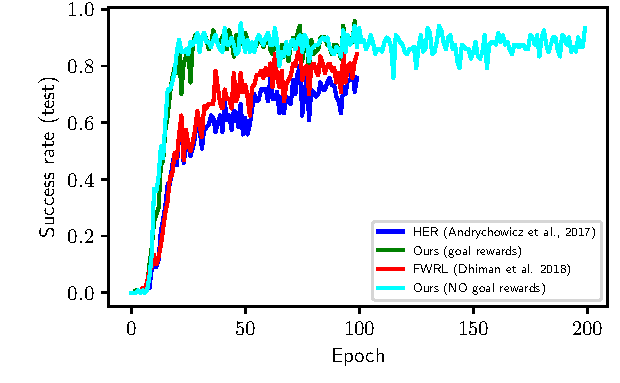
\includegraphics[width=\frac\columnwidth]{media/res/6efc1de-path_reward_low_thresh_chosen-FetchPickAndPlacePR-v1-dqst/epoch-test/success_rate.pdf}\\
  \label{fig:path-reward-fetch}%
  \caption{Effect of path reward on convergence in case of different algorithms
on Fetch tasks. Our method is able achieve similar performance even without the
goal rewards. Since our method without goal-rewards does not need reward
recomputation, we vastly outperform other methods in terms of reward sample
complexity.}%
\end{figure}
\begin{figure}
  \def\frac{0.24}
  \rotatebox{90}{{\tiny \hspace{1em} \color{blue}{Hand Reach}}}%
  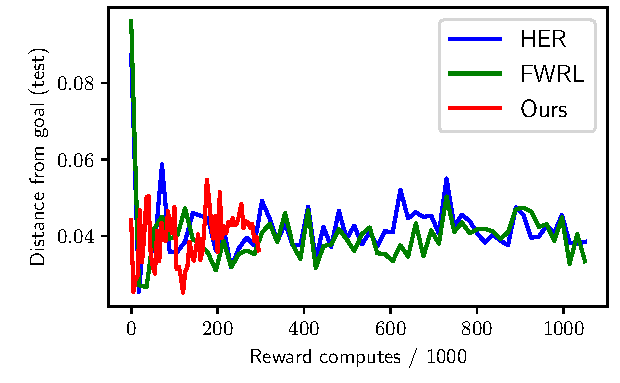
\includegraphics[width=\frac\columnwidth]{media/res/6efc1de-path_reward_low_thresh_chosen-HandReachPR-v0-dqst/reward_computes-test/ag_g_dist.pdf}%
  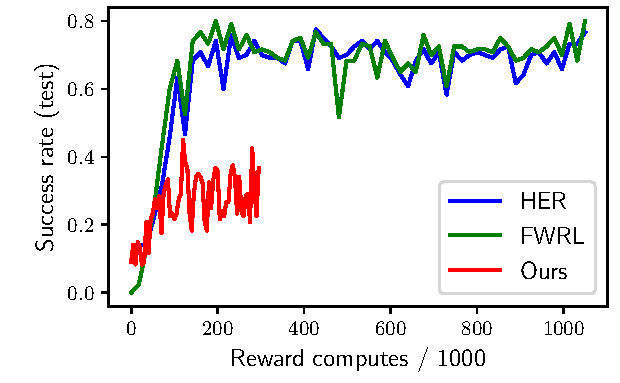
\includegraphics[width=\frac\columnwidth]{media/res/6efc1de-path_reward_low_thresh_chosen-HandReachPR-v0-dqst/reward_computes-test/success_rate.pdf}%
  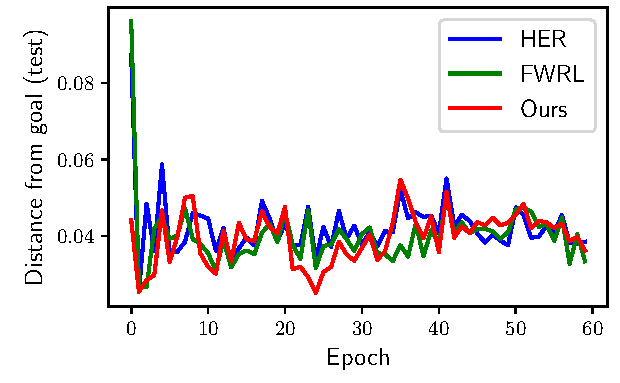
\includegraphics[width=\frac\columnwidth]{media/res/6efc1de-path_reward_low_thresh_chosen-HandReachPR-v0-dqst/epoch-test/ag_g_dist.pdf}%
  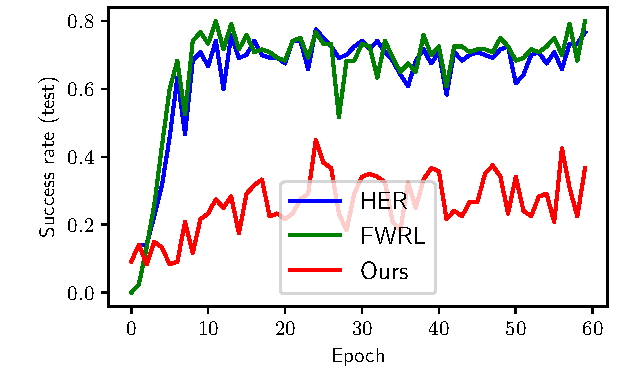
\includegraphics[width=\frac\columnwidth]{media/res/6efc1de-path_reward_low_thresh_chosen-HandReachPR-v0-dqst/epoch-test/success_rate.pdf}\\
  \rotatebox{90}{{\tiny \hspace{1em} \color{blue}{Hand Block Rotate}}}%
  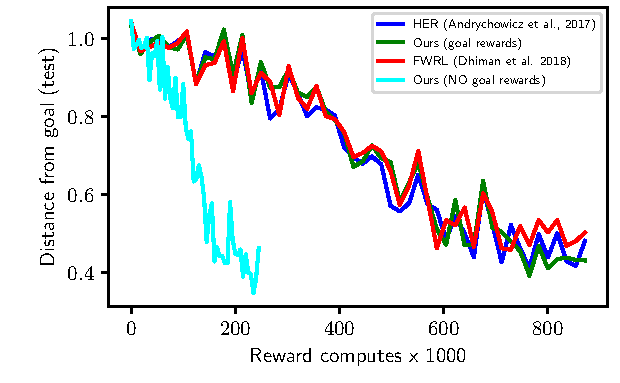
\includegraphics[width=\frac\columnwidth]{media/res/6efc1de-path_reward_low_thresh_chosen-HandManipulateBlockRotateXYZPR-v0-dqst/reward_computes-test/ag_g_dist.pdf}%
  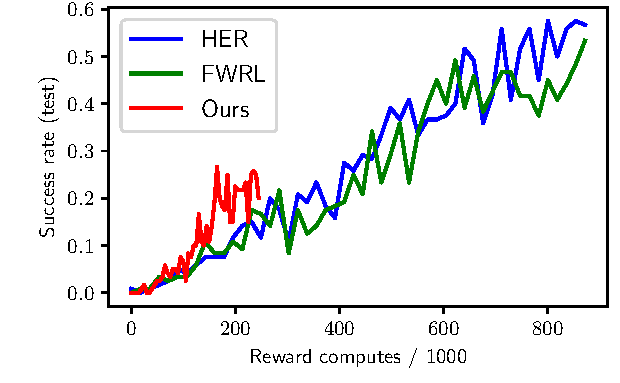
\includegraphics[width=\frac\columnwidth]{media/res/6efc1de-path_reward_low_thresh_chosen-HandManipulateBlockRotateXYZPR-v0-dqst/reward_computes-test/success_rate.pdf}%
  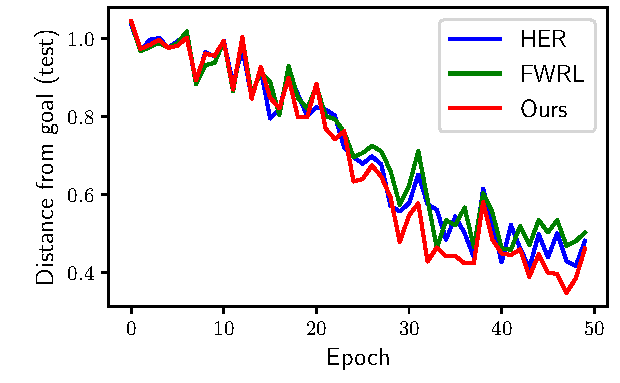
\includegraphics[width=\frac\columnwidth]{media/res/6efc1de-path_reward_low_thresh_chosen-HandManipulateBlockRotateXYZPR-v0-dqst/epoch-test/ag_g_dist.pdf}%
  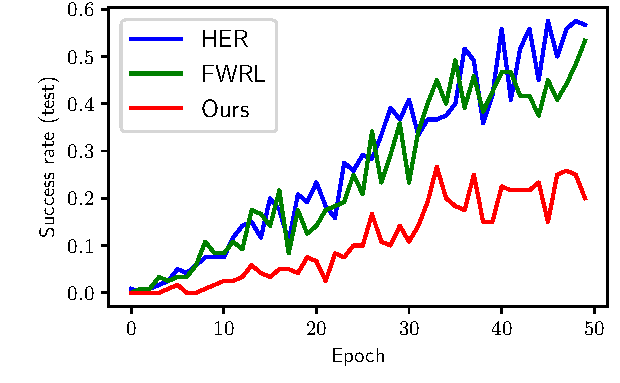
\includegraphics[width=\frac\columnwidth]{media/res/6efc1de-path_reward_low_thresh_chosen-HandManipulateBlockRotateXYZPR-v0-dqst/epoch-test/success_rate.pdf}\\
  \rotatebox{90}{{\tiny \hspace{1em} \color{blue}{Hand Egg}}}%
  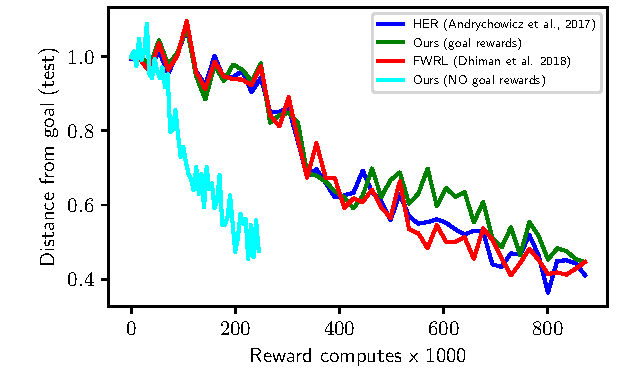
\includegraphics[width=\frac\columnwidth]{media/res/6efc1de-path_reward_low_thresh_chosen-HandManipulateEggFullPR-v0-dqst/reward_computes-test/ag_g_dist.pdf}%
  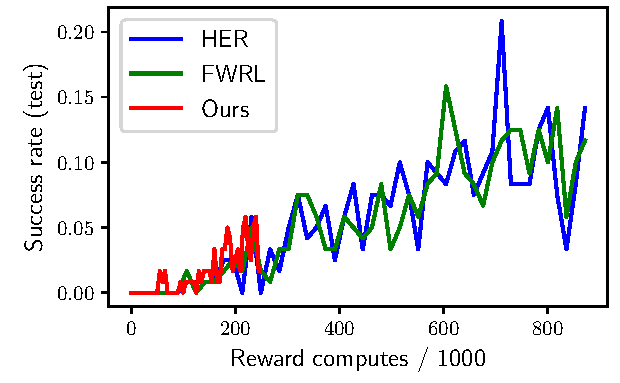
\includegraphics[width=\frac\columnwidth]{media/res/6efc1de-path_reward_low_thresh_chosen-HandManipulateEggFullPR-v0-dqst/reward_computes-test/success_rate.pdf}%
  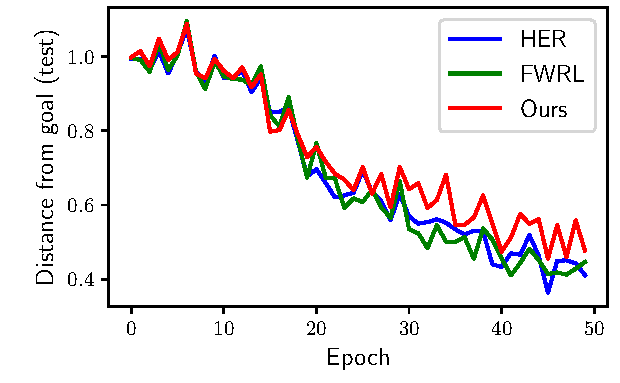
\includegraphics[width=\frac\columnwidth]{media/res/6efc1de-path_reward_low_thresh_chosen-HandManipulateEggFullPR-v0-dqst/epoch-test/ag_g_dist.pdf}%
  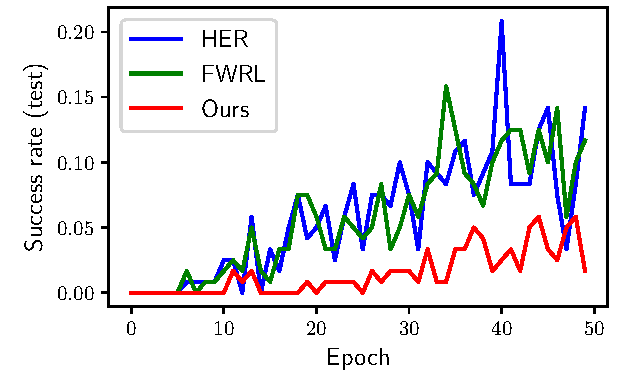
\includegraphics[width=\frac\columnwidth]{media/res/6efc1de-path_reward_low_thresh_chosen-HandManipulateEggFullPR-v0-dqst/epoch-test/success_rate.pdf}\\
  \rotatebox{90}{{\tiny \hspace{1em} \color{blue}{Hand Pen Rotate}}}%
  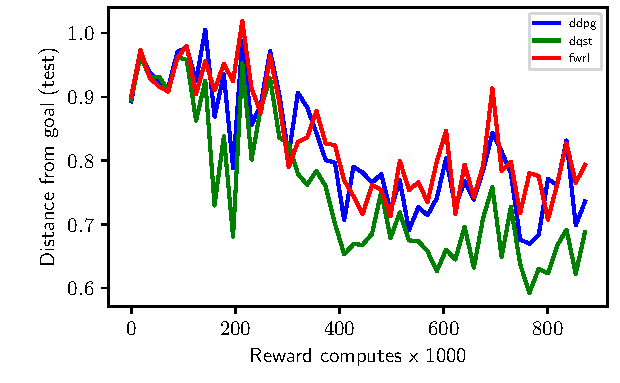
\includegraphics[width=\frac\columnwidth]{media/res/6efc1de-path_reward_low_thresh_chosen-HandManipulatePenRotate-v0-dqst/reward_computes-test/ag_g_dist.pdf}%
  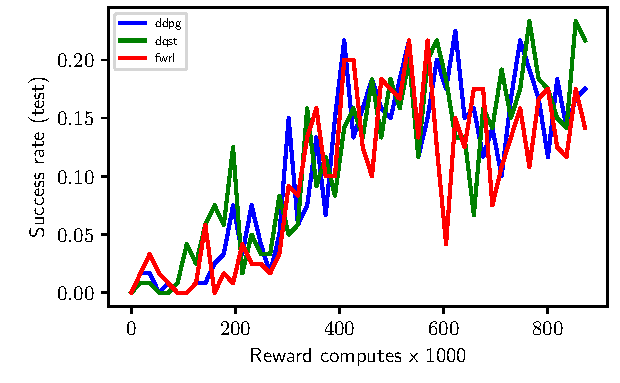
\includegraphics[width=\frac\columnwidth]{media/res/6efc1de-path_reward_low_thresh_chosen-HandManipulatePenRotate-v0-dqst/reward_computes-test/success_rate.pdf}%
  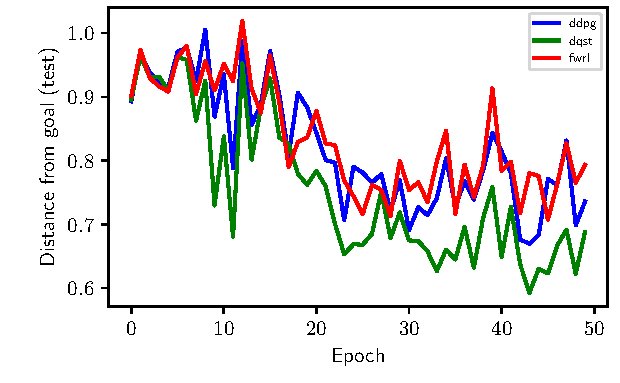
\includegraphics[width=\frac\columnwidth]{media/res/6efc1de-path_reward_low_thresh_chosen-HandManipulatePenRotate-v0-dqst/epoch-test/ag_g_dist.pdf}%
  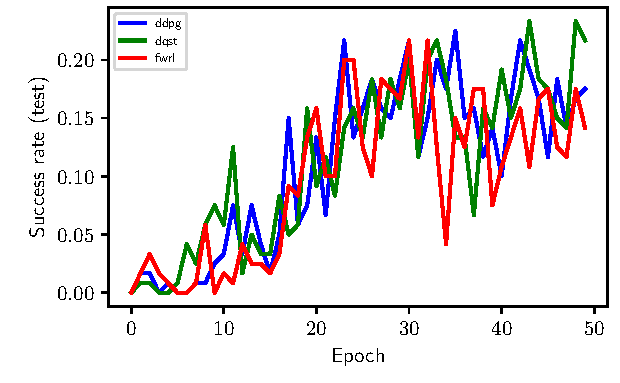
\includegraphics[width=\frac\columnwidth]{media/res/6efc1de-path_reward_low_thresh_chosen-HandManipulatePenRotate-v0-dqst/epoch-test/success_rate.pdf}\\
  \label{fig:path-reward-hand}%
  \caption{Effect of path reward on convergence in case of different algorithms
on Hand tasks. Our method is able achieve similar performance even without the
goal rewards. Since our method without goal-rewards does not need reward
recomputation, we vastly outperform other methods in terms of reward sample
complexity.}%
\end{figure}%
% 